% !TeX encoding = UTF-8
% !TeX spellcheck = en_US
% !TeX program = lualatex
%\directlua{pdf.setminorversion(6)}
\documentclass[a4paper,11pt,twoside,openright,onecolumn,titlepage,openbib,hluatex]{book}

\makeatletter
\usepackage[a-3b]{pdfx}
\pdftrue
\usepackage[draft]{HDRdfolio} 

% ********************************** Preamble **********************************
% Preamble: Contains packages and user-defined commands and settings
% !TeX encoding = UTF-8
% !TeX spellcheck = en_US
% !TeX root = ../hdr_dfolio.tex

\usepackage[draft]{HDRdfolio}  
\usepackage{dfNotations}  

\geometry{hmargin=2.5cm,vmargin=2cm,includeheadfoot,headheight=14pt,headsep=1.5em,footskip=1.5em}

\makeglossary
\makeindex

% Acronym
\NewAcro{ENSI}{\French{École Nationale Supérieur d’Ingénieurs}}
\NewAcro{INSA}{\French{Institut National des Sciences Appliquée}}
%\NewAcro{CVLacr}
\def\CVL{\French{Centre Val de Loire}}

\NewAcro{PRISME}{\French{Laboratoire Pluridisciplinaire de Recherche en Ing\'enierie des Syst\`emes, M\'ecanique, \'Energ\'etique}\protect\GlsSeeMore{glos:PRISME}}
\newglossaryentry{glos:PRISME}{type=glg,
  name=PRISME Laboratory,
  description={The \PRISMEshort Laboratory is from \French{Université d'Orléa,s} and \INSAshort \CVL (EPRES 4229), \url{http://www.univ-orleans.fr/PRISME}.
    The \PRISMEshort laboratory seeks to carry out multidisciplinary research in the general domain of engineering sciences over a broad range of subject areas, including combustion in engines, energy engineering, aerodynamics, the mechanics of materials, image and signal processing, automatic control and robotics.  }
}
\NewAcro{NANOMA}{Nano-Actuators and Nano-Sensors for Medical Applications\protect\GlsSeeMore{glos:NANOMA}}
\newglossaryentry{glos:NANOMA}{type=glg,
  name=NANOMA project,
  description={The \NANOMAshort project is an European project funded under FP7-ICT-2007.3.6, Micro/nanosystems, coordinated by Professor Antoine Ferreira, \French{Université d'Orléans}. The NANOMA project aims at proposing novel controlled nanorobotic delivery systems which will be designed to improve the administration of drugs in the treatment and diagnosis of breast cancer.}
}

\NewAcro{ANR}{\French{Agence Nationale de la Recherche}}% National Agency for Research
\NewAcro{PIANHO}{Innovative Haptic Instrumental platform for 3D Nano-manipulation\protect\GlsSeeMore{glos:PIANHO}}
\newglossaryentry{glos:PIANHO}{type=glg,
  name=PIANHO project,
  description={The \PIANHOshort project is an ANR P3N (2009) project. The objective has been to design a micromanipulation platform capable of pick, hold and place nano-objects in the synchrotron radiation beam of the ESRF, Grenoble, France.}
}



\NewAcro{RMN}{r\'esonance magn\'etique nucl\'eaire}
\NewAcro{IRM}{imagerie  par r\'esonance magn\'etique}
\NewAcro{MRN}{\English{magnetic resonance navigation}}
\NewAcro{EMA}{actionnement \'electromagn\'etique}
\NewAcro{TMMC}{\English{Therapeutic magnetic microcarriers}}
\NewAcro{SPIO}{\English{superparamagnetic particles iron oxide}}

\NewAcro{MRA}{\English{Magnetic resonance angiography}}
\NewAcro{MRI}{\English{Magnetic Resonance Imaging}}
\NewAcro{IRIS}{Institut de Robotique et des Syst\`emes Intelligents, \url{http://www.iris.ethz.ch}}
\NewAcro{ETH}{Institut F\'ed\'eral de Technologie de Zurich (Suisse), \url{http://www.ethz.ch}}
\NewAcro{AMiR}{Division Microrobotics and Control Engineering de l'Universit\'e d'Oldenburg, Allemagne, dirig\'e par le professeur Sergej Fatikov, \url{http://www.amir.uni-oldenburg.de}}


\NewAcro{DDL}{degr\'es de libert\'e}
\NewAcro{RF}{radiofr\'equence}



\NewSymb[sort=c8]{Reynolds}{\ensuremath{\mathrm{R}_{e}}\xspace}{\NoUnit}{Nombre de Reynolds}


% correct bad hyphenation here
\hyphenation{op-tical net-works semi-conduc-tor micro-robot}



\author{David FOLIO}
\title{Biomedical MicroRobotics}
\date{\today}

\providecommand{\RefChapI}{\ChapRef{I}}
\providecommand{\RefChapII}{\ChapRef{II}}
\providecommand{\RefChapIII}{\ChapRef{III}}
\providecommand{\RefChapIV}{\ChapRef{4}}
\providecommand{\RefChapV}{\ChapRef{5}}
\providecommand{\RefAnnexeA}{\ChapRef{A}}
\providecommand{\RefAnnexeCV}{\ChapRef{CV}}\let\RefCV\RefAnnexeCV
\providecommand{\RefAnnexeRef}{\ChapRef{MyRef}}\let\RefMyRef\RefAnnexeRef

\makeatother

\begin{document}

\thispagestyle{empty}
\maketitle
\thispagestyle{empty}
\clearemptydoublepage

\frontmatter
\tableofcontents
\clearemptydoublepage
\listoffigures
\clearemptydoublepage
\listoftables%

\mainmatter


% !TeX encoding = UTF-8
% !TeX spellcheck = en_US
% !TeX root = ../hdr_dfolio.tex

\Chapitre[1]{Context of Activities}
% !TeX encoding = UTF-8
% !TeX spellcheck = en_US
% !TeX root = ../hdr_dfolio.tex
\Chapitre[ChapII]{Chapter 2}

\Appendix
%\addcontentsline{toc}{part}{\appendixname}

% $Id$
% !TeX encoding = UTF-8
% !TeX spellcheck = en_US
% !TeX root = ../hdr_dfolio.tex

% ---------------------------------------------------------------------------------
%% My (long) resume ---------------------------------------------------------------
\Chapitre[CV]{Resume}
\glsadd{MRI}
\glsadd{PRISME}

\HDRskip
%\vspace*{-2em}


\noindent
\begin{minipage}{.64\linewidth-1em}
  \begin{minipage}{80pt}\draftHrule\raggedright
   \framebox{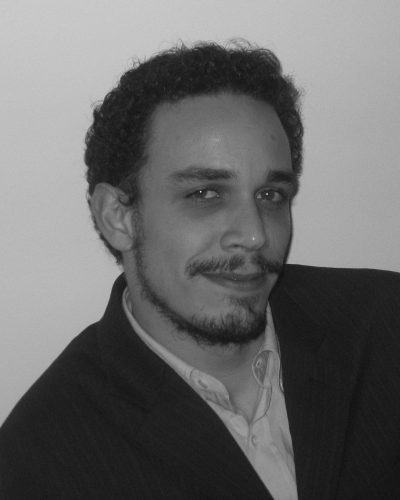
\includegraphics[width=\linewidth-10pt]{fig/david_folio}}
 \end{minipage}\hskip0.5ex plus0pt
  \begin{minipage}{\linewidth-82pt-1ex}\draftHrule
    \sffamily
    {\Huge\bfseries\upshape\scshape
      David FOLIO} \\
    {\smaller Born on the 17th September 1979},
    {\smaller French nationality}
    \\[0.5ex]
    {\Large\mdseries\slshape\color{blue1}
      Associate Professor (tenured)} \par\vskip1em plus1fill
    \begin{flushright}
      {\itshape\small\color{blue3}
        Robotic and Micro/Nano-robotic\linebreak[3] for biomedical and health-care\,applications}
    \end{flushright} 
  \end{minipage}
\end{minipage}\hskip0.5ex plus1fill
\begin{minipage}{.34\linewidth}\draftHrule
  \small\sffamily\mdseries\upshape
    {\normalsize\INSA \CVL,} \\
    {\French{Universit\'e d'Orl\'eans}, \PRISMEshort EA 4229} \\
    {Campus de Bourges,  88 bd Lahitolle}\\
    {CS 60013}\\
    {F-18022 Bourges cedex; France} \\
    \marvosymbol{84}~{+33~(0)~2\,48\,48\,40\,75}\\
    \marvosymbol{117}~{+33~(0)~2\,48\,48\,40\,50}  \\
    \marvosymbol{66}~\emaillink{david.folio@insa-cvl.fr} 
\end{minipage}

\HDRskip
%\vspace*{-2em}

% ---------------------------------------------------------------------------------
% SECTION -------------------------------------------------------------------------
\section{Curriculum Vit\ae}


\subsection{Current position and responsibilities}
\noindent
\begin{tabularx}{\linewidth-1em}{@{}>{\raggedleft}p{3.133\parindent}@{\hspace{2ex}}X@{}}
  \datestyle {Since 2008} 
  & \degreestyle{Associate Professor} \French{(ma\^itre de conférences,  61\up{\`eme} CNU section)}\newline
  \affiliationstyle{{\INSA \CVL}, {Universit\'e d'Orl\'eans}, {\PRISME Laboratory EA 4229} {Bourges, France}} %\newline
  \begin{description}
    \smaller
    \item[Teaching]  { member of the teaching team of the Industrial Risk Control (MRI\footnote{In French \French{Ma\^itrise des Risques Industriels (MRI)}.}), of the Energy, Risks, and Environment (ERE),  and of the Sciences and Techniques for Engineers (STPI\footnote{In French \French{Science et Technique pour l'Ingénieur (STPI)}.}) departments;}
    \item[Research] member of the Robotic team of the IRAuS unit of \PRISME Laboratory
  \end{description}
  %& {\smaller \textbf{\sffamily Teaching}: \\
 % & {\smaller \textbf{\sffamily {Research}}: member of the Robotic team of the IRAuS unit of \PRISME Laboratory.} 
  \\[1ex]
  \datestyle {Since 2014}
  & { in charge of the Nuclear Energy option of the 5\up{th} year (engineer's degree) of the Industrial Risk Control (MRI) department.}\\[1ex]
  \datestyle {Since 2017}
  & {  referent of \enquote{racism and antisemitism}.}\\[1ex]
  \datestyle {Since 2017}
  & {elected  member of the Energy, Risks and Environment (ERE) department council.}
\end{tabularx}
\par\nobreak\bigskip

%\vspace*{-2em}
\subsection{Experience and Graduate Education}
\noindent
\begin{tabularx}{\linewidth-1em}{@{}>{\raggedleft}p{3.133\parindent}@{\hspace{2ex}}X@{}}
 \datestyle {Oct.\,2007 Aug.\,2008} 
    & \degreestyle{Post-Doctorate}  
    {at Inria de Rennes Bretagne Atlantique\footnote{French Institute for Research in Computer Science and Automation (French: \French{Institut national de recherche en informatique et en automatique}).  \url{https://www.inria.fr/centre/rennes}}, {Rennes, France}} \newline
     {\smaller Research conducted in Lagadic team, supervised by François Chaumette.}
  \\[1ex]
  \datestyle {Feb.\,2007 Aug.\,2007} 
    & \degreestyle{Teaching assistant}: {\smaller\French{Attaché Temporaire d'Enseignement et de Recherche (ATER)}}
    {at Paul Sabatier University of Toulouse, {France}} 
  \\[1ex]
  \datestyle {Feb.\,2004 Jul.\,2007} 
    & \degreestyle{Doctorate}
    {at LAAS-CNRS, {Toulouse, France}} \newline
    {\smaller \PhD Thesis in Robotic control, directed by Viviane Cadenat, entitled
      \enquote{Multi-sensor-based control strategies and visual signal loss management for
        mobile robots navigation}.}
  \\[1ex]
  \datestyle {2003--2004} 
  & \degreestyle{Master of Science} \French{(DESS)} Intelligent Systems
  {at Paul Sabatier University of Toulouse, {France}} 
  \\[1ex]  
  \datestyle {2002--2003} 
  & \degreestyle{Master of Advanced Studies} \French{(DEA)} Computer Sciences
  {at Paul Sabatier University of Toulouse, {France}} 
  \\[1ex]
  \datestyle {1999--2002} 
  & Scholarship \French{(IUP\footnote{In French \French{Institut Universitaire Professionnalisé} (IUP)}, L2-M1)} on Intelligent Systems
  {at Paul Sabatier University of Toulouse, {France}} 
  \\[1ex]
\datestyle {1997--1999} 
& \degreestyle{Bachelor's degree} \French{(DEUG, L1-L2)} in Science and Technology for the Engineer,
{at University of Reunion Island, {France}} 
\end{tabularx}


\subsection{Professional Activities}
\noindent
\begin{tabularx}{\linewidth-1em}{@{}>{\raggedleft}p{3.133\parindent}@{\hspace{2ex}}X}
  \datestyle{Since 2015}
    &{Member of the program committee of the \emph{International Conference on Robotics, Manipulation, and Automation at Small Scales} (MARSS)} \\
  \datestyle{Since 2013}
    &{Editorial Board member of the \emph{International Journal of Advanced Robotic Systems} (IJARS).}\\
  \datestyle{Since 2005}
    &{IEEE member (SM'05, AM'08, M'12)}\\[2ex]
  \datestyle{Regular Reviewer}
  &\vspace*{-1ex} %\relsize{-0.5}
  \begin{itemize}
    \item \emph{IEEE Transactions on Robotics} (TRO);
    \item \emph{IEEE Transactions on Biomedical Engineering} (TBME);
    \item \emph{{IEEE/ASME} Transactions on Mechatronics} (TMECH);
    \item \emph{{IEEE} Transactions on Automation Science and Engineering} (TASE);
    \item \emph{International Journal of Advanced Robotic Systems} (IJARS);
    %\item Journal Europ\'een des Syst\`emes Automatis\'es;
    \item \emph{{IEEE} International Conference on Robotics and Automation} (ICRA);
    \item \emph{{IEEE/RSJ} International Conference on Intelligent Robots and Systems} (IROS);
    \item \emph{IEEE International Conference on Biomedical Robotics and Biomechatronics} (BioRob);
    %\item {IEEE} Engineering in Medicine and Biology Society (EMBC);
    %\item Conf\'erence Internationale Francophone d'Automatique (CIFA);
    % \item {IEEE} Engineering in Medicine and Biology Society (EMBC);
    %\item International Conference on Biomedical Engineering and Biotechnologie (iCBEB);
  \end{itemize}\\  
  \datestyle{Awards} & French outstanding research award (PEDR 2014-2018)
\end{tabularx}


\HDRskip

%\pagebreak[3]


% ---------------------------------------------------------------------------------
% SECTION -------------------------------------------------------------------------
\section{Teaching Activities}\label{sec:CV:teaching}

\subsection{Teaching}

My overall teaching activities  have been solely related with the 61\up{st} CNU section\footnote{\label{foot:CV:CNU}\French{Conseil national des universités} (CNU). \url{http://www.cpcnu.fr}} which regroups scientific disciplines from control, computer engineering and signal processing.
I taught these teaching as a temporary teacher (\SI{3}{\years}), teaching assistant (ATER, \SI{1}{\year}), and then as associate professor (\SI{10}{\years}).
These different experiences are presented in the following.

\subsubsection{Before tenure}
I have started teaching as a temporary teacher at the Paul Sabatier University of Toulouse, France, during my doctorate (2004-2006).
Next, I have pursued as teaching assistant, specifically  in French \EFrench{Attaché Temporaire d'Enseignement et de Recherche} (ATER, 2007) for  the Paul Sabatier University of Toulouse.
My teachings were then mainly in the fields of robotics, control theory, image processing and real-time systems for students from bachelor's to master's degrees.
These global teaching experiences have led to a total volume of \SI{308}{\hETD}\footnote{\label{foot:CV:hETD}\glsreset{HETD}\glsdesc[hyper=false]{HETD}}.

These activities were my first experience in high-graduate education.
Those opportunities  highlighted my interest in the scientifics knowledge transmission. 
They also allowed me to be familiarized with the different forms of teachings.
Indeed, I had then the opportunity to supervise not only tutorials (TD), practical work (TP), and long-term projects  (BE); but also few courses.
Especially, I also helped the teaching team by writing some TP contents, and  in the students evaluation.
This first experience confirmed my interest in teaching, leading me logically to apply for an associate professor position.

\subsubsection{Since tenured}
\glsreset{INSA}
I was recruited as Associate Professor  in September 2008 for the 61\up{st} CNU\footnoteref{foot:CV:CNU} section.
Untill now, my teaching activities have been mainly held at  \INSA \CVL on the Bourges campus.
The \INSA \CVL was established in 2014 following the merger of the Val de Loire ENI (National Engineering School) and Bourges ENSI (Graduate Engineering School).
With 200 members of staff (teachers, research professors, administrative and technical staff) the Institute trains 1500 students on its two campuses in Blois and Bourges, France. 
The Institute awards four engineering degrees:
\begin{enumerate}
  \item Industrial Risk Control (MRI) in Bourges;
  \item Information Technology and Cybersecurity (STI)   in Bourges; 
  \item Energy, Risk and the Environment (ERE) together with the Cher Chamber of Commerce and Industry (CCI) Hubert Curien CFSA (Apprentice Further Training Centre) in Bourges;
  \item Industrial Systems Engineering (GSI) in Blois
\end{enumerate}
The Institute was extended in 2015 when it absorbed the National Graduate School for Nature and Landscape, which has now become the "School for Nature and Landscape" department. 
Like all of the \INSA engineering schools, the first two years, that are common to each engineering degrees, is embedded in the Sciences and Techniques for Engineers (STPI) department.
It can been noticed, that the ERE department trains engineers through apprenticeship training
This program is  based on a partnership between the \INSA \CVL and Hubert Curien CFSA (Apprentice Further Training Centre), which has been an expert in delivering apprenticeship-based training for over 20 years.


\SkipAndBreak

As member of the teaching team on the campus in Bourges of \INSA \CVL, I am mainly involved in the students formation of the Industrial Risk Control (MRI), of the  Energy, Risk and the Environment (ERE), and of the  Sciences and Techniques for Engineers (STPI) departments. 
Specifically, after having started with teaching of  electronics and electrical engineering, I have participated or organized lessons on  signal processing, sensors, control and robotics.
%
These various teaching experiences imply very different pedagogical tasks.
Especially, those tasks are depending on the type of intervention: courses (C), tutorials (TD), practical works (TP), tutored projects (P), long-term project team work (BE); but also according to the different degrees of scientific maturity and specialization of the concerned students, \ie  from bachelor's to master's degrees level.
\autoref{tab:teaching} illustrates a synthetic overview of my different teaching discipline showing the degree, the number of students, and the face-time hours.
In particular, I am especially involved in the implementation of the teachings materials, and to support the teaching assistants for the disciplines for which I am in charge.
%
\begin{table}[tb]
  \centering
  \caption{Overview of the various learned discipline since tenured as associate professor.}\label{tab:teaching}
  \begin{tabular}{|>{\raggedleft}m{8em}|c|r|r|r|r|r|c|c|}
    \hline 
    \multirow{2}{=}{\sffamily Discipline} & \multirow{2}{2.33em}{\sffamily LMD} & \multirow{2}{3.66em}{\sffamily Students} & \multicolumn{4}{c|}{\sffamily Face time} & \multirow{2}{2.5em}{\sffamily Dept.} & \multirow{2}{2.5em}{\sffamily Resp.} \\ 
     &  &  & C & TD & TP & P/BE  & &  \\     \hline 
    Electrokinetics 
    &  L1 & 100 & 18h00 & 24h00  &  &  & STPI & Yes \\ 
    \hline 
     \multirow{2}{=}{\raggedleft Analogue electronics}
     & L2 & 80 &   8h00 & 32h00 &  & &  STPI & Yes  \\ 
     & L3 & 70 &  10h40 & 10h40 & 6h00 & &  MRI  & Yes  \\ 
    \hline 
    \multirow{2}{=}{\raggedleft Electrical engineering}
    & L3 & 70 &  10h40 & 10h40 &  & &  MRI & Yes  \\ 
    & M1 & 78 &   8h00 & 14h00 &  & &  ERE & Yes  \\ 
    \hline 
    Control& M1 & 78 & 6h00 & 10h00 &  & &  ERE & Yes  \\ 
    \hline 
    Signal processing & M1 & 20 & 10h40 & 10h40 &  & &  MRI & Yes  \\ 
    \hline 
    Diagnostic & M1 & 20 & 10h40 & 10h40 &  & &  MRI & Yes  \\ 
    \hline 
    Sensors& L3 & 70 &  & 10h40  &  & &  MRI & No  \\ 
    \hline 
    Robotic& M2 & 20 &  4h00 &  &  & & MARS & No \\ 
    \hline  
    SA project& M1 & 2 &  &  &  &  5h20 &   MRI & No \\ 
    \hline 
    SI project& M1 & 10 &  &  &  &  14h20 &   MRI & No  \\ 
    \hline \hline 
    \multicolumn{3}{|r|}{\sffamily\textbf{Total} (face time)}& 86h40 & 133h20 & 6h00 & 19h40    \\ \cline{1-7}
  \end{tabular}

\begin{flushleft}\footnotesize\footnoterule
\begin{description}[format=\sffamily]
  \item[LMD] The bachelor's, master's, doctorate system (in French \French{Licence-Master-Doctorat}) designed by the Bologna Process, with 
  \begin{itemize}
    \item L1-L3: from the 1\up{st} to the 3\up{rd} year bachelor's degree;
    \item M1-M2: from the 1\up{st} to the 2\up{nd} year master's degree;
  \end{itemize}
  \item[Students] are the average number of students.
  \item[C, TD, TP, P] refer to face time hours for courses (C), tutorials (TD), practical works (TP), tutored projects (P).
  \item[Dept.] refers to the department of \INSA \CVL, that is
  Sciences and Techniques for Engineers (STPI),
  Industrial Risk Control (MRI),
  Energy, Risks and the Environment (ERE). \linebreak[3]{Further details are available on-line at: \url{http://www.insa-centrevaldeloire.fr}}.
  \item[Resp.] specifies the case where I am in charge of the discipline, especially with the implementation of the teaching materials.
  \item[SA and SI projects] refer to the Advanced Systems (SA) advanced module, and the Industrial System (SI) project  in the 4\up{th} year (M1).
\end{description}
\hrule
\end{flushleft}
\end{table}
%
\begin{figure}[tbh]
  \centering
  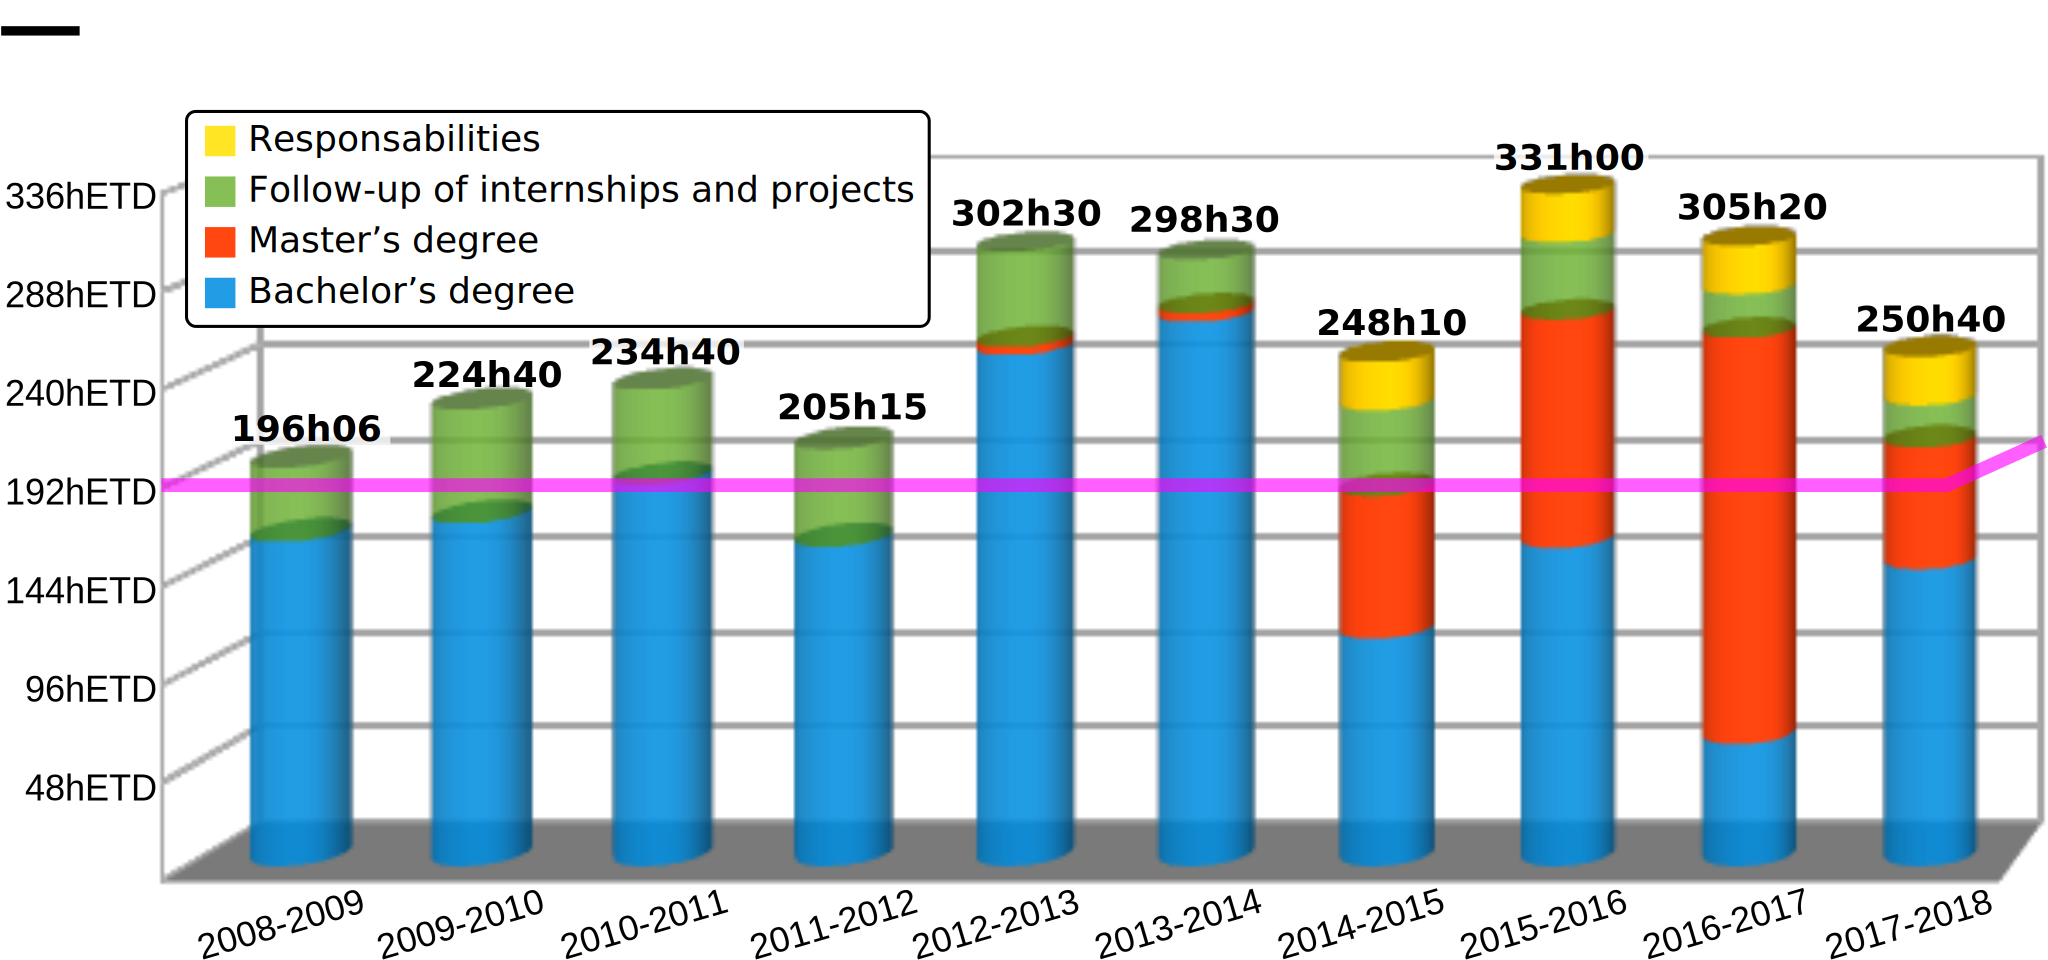
\includegraphics[scale=1]{fig/appendixCV/teaching_charge} %
  \caption[Teaching load progress]{Teaching load progress expressed in \enquote{equivalent TD hours}  (see \autoref{foot:CV:hETD}).
   My average teaching load is about \SI{280}{\hETD}.
  The line at \SI{192}{\hETD} is the minimum  teaching duty to be achieved.}
  \label{fig:teaching_charge}
\end{figure}

\medskip

Since tenured as associate professor, my average teaching load is about \SI{280}{\hETD}\footnoteref{foot:CV:hETD}.
This activity load is varied depending on the recruitment and the choice of engineering students in the different departments in which I intervene. 
In particular, the hours performed in tutorials (TD), practical works (TP) or  projects (P) depend on the number of groups (\ie from 2 to 4 groups), especially for the   bachelor's degrees (L1-L3).
\autoref{fig:teaching_charge} presents my teaching duty timeline progress expressed in \si{\hETD}  since tenured as Associate Professor.

Furthermore, some key events in the life of the Institute have also influenced my teaching loads (see also \autoref{fig:timeline}).
For instance, from 2011, following the integration of the former Bourges \ENSI  in the \INSA group,   I took part in the electronics training for the new preparatory cycle.
In parallel, since 2011, after the ERE department creation,  I have also started to form the apprentices engineers to electrical engineering.
In addition, various responsibilities entrusted to me have also influenced my teaching duties, and are presented hereafter. 

\subsection{Responsibilities}

%Plusieurs "obligations de services" sont liées à la fonction de maître de conférences : la participation aux jurys d

In addition to teaching tasks, different  obligations are related to the mission of teaching-researchers in France.
Thus, I am involved in the life of the Institute. 
Especially, I contribute at a local level to the scientific animations (eg., organization of laboratory visits), transfer and training-research links. 
Furthermore, since my tenure, I participate in the juries of our engineering students.
Similarly, since our establishment have joint the \INSA group, I also contribute to select and interview the applying students (about 15 students/year).
Between 2009 and 2013, I have been member of the Hygiene and Security committee of the \ENSI of Bourges.

Since September 2014, I am in charge of the Nuclear Energy option of the 5\up{th} year (engineer's degree) of the Industrial Risk Control (MRI) department. 
As such, I coordinate the specific lessons of the option by selecting and recruiting external professional contractors. 
I also organize visits (power station, simulator, etc.) for the engineering students of the option.
 
In March 2017, the direction of the \INSA \CVL  given to me the mission of referent \enquote{racism and antisemitism}.
Since November 2017, I am an elected member of the ERE  department council.
 
%\SkipAndBreak

%\pagebreak[3]
\glsadd{MRI}
\glsadd{ANR}


% ---------------------------------------------------------------------------------
% SECTION -------------------------------------------------------------------------
\section{Research Activities}

\subsection{Scientific Projects}\label{sec:CV:projects}
My research activities regularly lead me to collaborate in various scientific projects.
In particular, these projects aim to obtain funds to either recruit \PhD students, to design or improve experimental testbeds, as well as to help some scientific cooperations.
The different projects in which I have been involved are listed below, specifying my role and the obtained fundings.
Let us notice that all of these  projects have been subject to a process with a deep scientific review.

\subsubsection[European Union  and National Funding Projects]{European Union (EU) and National Funding (ANR) Projects}

\begin{enumerate}[leftmargin=3em,format={\sffamily\bfseries\smaller\color{blue2}},label={[EU\arabic*]}]
  \item{}\textsf{NANOMA}: \label{proj:NANOMA} \glsdesc[hyper=false]{NANOMA}
  \begin{description}
    \item[Date] 06/2008 -- 10/2011
    \item[Funding] \SI{3.3}{\mega\euro}, supported by the European Commission
    \item[Summary] \glsdesc[hyper=false]{glos:NANOMA}
    \item[Role] co-responsible of the workpackage WP4: ``{Object Tracking, Planning and Control in \MRIshort}''.
  \end{description}
\end{enumerate}

  \medskip
  
\begin{enumerate}[leftmargin=3em,format={\sffamily\bfseries\smaller\color{blue2}},label={[ANR\arabic*]}]
  \item{}\textsf{PROSIT}: \label{proj:PROSIT}  \glsdesc[hyper=false]{PROSIT} 
  \begin{description}
    \item[Date] 01/2009 -- 09/2012
    \item[Funding] \SI{230}{\kilo\euro}, supported by  French national funding (\ANRshort\footnote{{\acrlong{ANR}} (ANR) is the French National Agency for Research.
      \hfill 
       \url{http://www.agence-nationale-recherche.fr}})
    \item[Summary] \glsdesc[hyper=false]{glos:PROSIT}
    \item[Role] co-responsible  of the workpackage WP5: ``{Visual Servoing}''.
  \end{description}


  \medskip
  \item{}\textsf{PROTEUS}: \label{proj:PROTEUS} \glsdesc[hyper=false]{PROTEUS} 
  and academics
  \begin{description}
    \item[Date] 12/2009 -- 12/2013
    \item[Funding] \SI{2.1}{\mega\euro}, supported by  French national funding (\ANRshort)
    \item[Summary]  \glsdesc[hyper=false]{glos:PROTEUS}
    To achieve the \PROTEUSshort project 12 partners have been involved.
    \item[Role] co-responsible  of the workpackage: ``{Young Challenge}''.
  \end{description}

\SkipAndBreak

  \item{}\textsf{PIANHO}: \label{proj:PIANHO}  \glsdesc[hyper=false]{PIANHO} %Innovative Haptic Instrumental platform for 3D Nano-manipulation
  \begin{description}
    \item[Date] 03/2010 -- 03/2014
    \item[Funding] \SI{761}{\kilo\euro}, supported by   French national funding (\ANRshort)
    \item[Summary] \glsdesc[hyper=false]{glos:PIANHO}
    \item[Role] co-responsible  of the workpackage: ``{Control of a Two-Fingered AFM-based Nano-manipulation System}''.
  \end{description}  
\end{enumerate}


%\SkipAndBreak[2]

\subsubsection{Cooperation Projects}\label{sec:CV:coll:proj}

\begin{enumerate}[leftmargin=3em,format={\sffamily\bfseries\smaller\color{blue2}},label={[PHC\arabic*]}]
  \item{}\textsf{PHC PROCOPE}: \label{proj:PROCOPE} Franco-Germain Hubert Curien\footnote{\PHC provides support for international scientific and technological exchange of the Ministry of Foreign Affairs. \url{https://www.campusfrance.org}} partnership
  \begin{description}
    \item[Date] 2010 -- 2011
    %\item[Funding] \SI{3.3}{\mega\euro}, supported by the European Commission
    \item[Summary]  Supervision and Control of an Improved \MRI Platform for Targeted Administration of Therapeutic Nanorobots.
    \item[Partnership] \glsdesc[hyper=false]{glos:AMiR}
  \end{description}

\SkipAndBreak
  \item{}\textsf{PHC PROCORE}: \label{proj:PROCORE} France--Hong-Kong Hubert Curien partnership
  \begin{description}
    \item[Date] 2014 -- 2015
    %\item[Funding] \SI{3.3}{\mega\euro}, supported by the European Commission
    \item[Summary]  Design, fabrication and characterization of the swim of enhanced helical microrobots.
    \item[Partnership] \glsdesc[hyper=false]{glos:MAE}
  \end{description}
\end{enumerate}

\subsubsection[Local Project]{Local Project (LP)}

\begin{enumerate}[leftmargin=3em,format={\sffamily\bfseries\smaller\color{blue2}},label={[LP\arabic*]}]
  \item{}\textsf{Nano-IRM}
  \begin{description}
    \item[Date] 09/2009 -- 08/2012
    \item[Funding] \SI{110}{\kilo\euro}, supported by \French{Région Centre Val de Loire}\footnote{Administrative region of France for Centre-Loire Valley. \url{http://www.regioncentre-valdeloire.fr}}, the Cher (18) departmental councils and the agglomeration comity of Bourges.
    \item[Summary] Supervision and Control of an Improved \MRI Platform for Targeted Administration of Therapeutic Nanorobots.
    This project supports the above \glsdisp{NANOMA}{NANOMA} project \ref{proj:NANOMA}, by providing the funding for the \PhD thesis of Karim~Belharet.
    \item[Role] co-supervision of the \PhD thesis of Karim~Belharet.
  \end{description}

  \medskip
  \item{}\textsf{MicroRob}
  \begin{description}
  \item[Date] 10/2013 -- 09/2016
  \item[Funding] \SI{110}{\kilo\euro}, supported by \French{Région Centre Val de Loire} and the agglomeration comity of Bourges.
  \item[Summary] Modeling and control of magnetic microcarrier for targeted cancer therapy.
  \item[Role] co-supervision of the \PhD thesis of Lyes~Mellal.
  \end{description}
  \medskip
  
  \item{}\textsf{\bfseries High Definition Echograph}
  \begin{description}
    \item[Date] 03/2017 -- 03/2018
    \item[Funding] \SI{50}{\kilo\euro}, supported by \French{Région Centre Val de Loire} 
    \item[Summary] Design of novel microrobotic platform with ultrasound probe vision.
    \item[Role] \textsl{Principal Investigator} (PI).
  \end{description}

\end{enumerate}

\SkipAndBreak

\subsection{Students Supervisions}\label{sec:CV:supervision}
My research activities as associate professor led to the supervision of graduate school students from master's to doctoral degrees.
Specifically, I had directly supervised 4 doctorate (3 defended theses and 1 on going) and 2 master theses.
In addition, I also had the opportunity to follow the research works of 5 external \PhD students.
The different students that  I have supervised or followed their works are listed below.


\subsubsection[PhD Students]{\PhD Students}\label{sec:CV:PhD}

\paragraph{Thesis in progress}\label{sec:CV:PhD:continue}

\begin{enumerate}[leftmargin=3em,format={\sffamily\bfseries\smaller\color{blue2}},label={[SUP\arabic*]}]
  \item{}\textsf{Ruipeng~Cheng}, 
  \begin{description}
    \item[Date] 11/2016 
    \item[Title] Predictive navigation of a magnetic microrobot:    instrumentation, control and validation
    \item[Supervision rate]  50\% with the Prof. Antoine Ferreira (\INSA \CVL) %[{\parbox[t]{1.75cm}{\raggedleft\smaller Supervision\\ Rate}}]
  \end{description}
  \SaveOrder
\end{enumerate}

\paragraph{Defended theses}\label{sec:CV:PhD:defended}

\begin{enumerate}[leftmargin=3em,format={\sffamily\bfseries\smaller\color{blue2}},label={[SUP\arabic*]}]
  \LoadOrder
  \item{}\textsf{Karim~Belharet}, 
  \begin{description}
    \item[Date] 11/2009 -- 10/2013
    \item[Title] Predictive navigation of a magnetic microrobot:    instrumentation, control and validation
    \item[Supervision rate] 50\% with the Prof. Antoine Ferreira (\INSA \CVL)
    \item[Publications] \cite{2010_biorob_belharet,2010_iros_belharet,2010_mitat_belharet,2011_advrob_belharet,2012_book_belharet,2012_iros_belhharet,2012_isot_belharet,2013_isot_belharet,2013_tbme_folio,2014_icra_belharet,2014_iros_belharet}
    \item[Position] Associate Professor at \French{École des Hautes Études d’Ingénieur}\footnote{French for private School of High Studies in Engineering, \url{http://centre.hei.fr}.} (HEI).
  \end{description}
  
  \medskip
  \item{}\textsf{Nabil~Amari}, 
  \begin{description}
    \item[Date] 11/2011 -- 08/07/2016
    \item[Title] Development  and Control of a Micro-Robotics Platform for the Synchronization of  a Light Beam
    \item[Supervision rate] 33.3\% with the Prof. Antoine Ferreira (\INSA \CVL)
    \item[Publications] \cite{2013_iros_amari,2013_isot_amari,2014_acc_amari,2014_ijo_amari,2014_iros_amari,encyclo_2016_amari}
    \item[Position] ???
  \end{description}
  
  \medskip
  \item{}\textsf{Lyès~Mellal}, 
  \begin{description}
    \item[Date] 11/2013 -- 07/12/2016
    \item[Title] Modeling and Control of Magnetic Microrobots for Therapeutic  Targeting
    \item[Supervision rate] 50\% with the Prof. Antoine Ferreira (\INSA \CVL)
    \item[Publications] \cite{2015_jnr_lyes,2015_com_mellal,2015_iros_mellal,2016_icra_mellal,2016_com_mellal,2016_marss_mellal,2016_tnb_lyes,2017_marss_mellal}
    \item[Position] 
  \end{description}
  \SaveOrder
\end{enumerate}

\SkipAndBreak

\subsubsection{External Students}
Hereafter, are mentioned only students follow-ups that has lead to a publication.
The mentioned dates correspond to the periods during which the follow-up of the students research was achieved.

\begin{enumerate}[leftmargin=3em,format={\sffamily\bfseries\smaller\color{blue2}},label={[EXT\arabic*]}]
  \item{}\textsf{Jungsik~Kim}, \PhD degree from Korea Advanced Institute of Science and Technology (KAIST), South Korea.
  \begin{description}
    \item[Date] 09/2009--12/2012 
    \item[Subject] A Study of Oocyte/Embryo Manipulation Using Microfluidics and Robotics.
    \item[Publications] \cite{2011_icra_kim,2012_tase_kim}
    \item[Position] Senior Research Engineer at LG Electronics, South Korea
  \end{description}
  
  \SkipAndBreak
  \item{}\textsf{Tao~Li}, \PhD degree from University of Rennes~1, France.
  \begin{description}
    \item[Date] 10/2009--02/2013 
    \item[Subject]Control of a tele-echography robot by visual servoing.
    \item[Publications] \cite{2014_isj_tao}
    \item[Position] Engineer at Total Immersion, Paris.
  \end{description}
  
  \SkipAndBreak
  \item{}\textsf{Christian~Dahmen}, \PhD degree from  University of Oldenburg, Germany.
  \begin{description}
    \item[Date] 2009--2016 
    \item[Subject]\MRI-based dynamic tracking and control of an untethered ferromagnetic microrobots.
    \item[Publications] \cite{2011_iros_folio,2012_iros_dahmen,2016_ijo_folio}
    \item[Position] N/A
  \end{description}
  \medskip
  
  \item{}\textsf{Bruno~Sarkis}, \PhD candidate at the Institut Jean Le Rond d'Alembert (IJLRA), UMR 7190, Pierre and Marie Curie University, Paris 6.
  \begin{description}
    \item[Date] 11/2014-- now 
    \item[Subject] Catalytic  microjet  modeling
    \item[Publications]\cite{2015_icra_sarkis,2018_jmems_sarkis}
  \end{description}
  
  \medskip
  \glsreset{ETH}
  \item{}\textsf{Bumjin Jang},  \PhD candidate at   \gls{MSRL} of  Swiss Federal Institute of Technology in Zurich\footnote{\glsdesc[hyper=false]{glos:MSRL}} (\acrshort{ETH}).
  \begin{description}
    \item[Date] 11/2016-- now 
    \item[Subject]  Catalytic locomotion of core-shell nanmotors.
    \item[Publications]\cite{2016_acsnano}
  \end{description}
  \SaveOrder
\end{enumerate}


\subsubsection{Masters Students}\label{sec:CV:Master}

\begin{enumerate}[leftmargin=3em,format={\sffamily\bfseries\smaller\color{blue2}},label={[MS\arabic*]}]
  \item{}\textsf{Kamel Ncir},  
  \begin{description}
    \item[Date] 03/2010--08/2010
    \item[Subject]  Modeling and control of a nano-positioning platform
  \end{description}
  
  \item{}\textsf{Nabil Amari},  
  \begin{description}
    \item[Date] 03/2011--08/2011
    \item[Subject]   Modeling and control of a nano-positioning platform
  \end{description}
\end{enumerate}

\SkipAndBreak[2]



\subsection{Scientific Collaborations}\label{sec:CV:coll}

My research work have led to various international and national collaborations.
These cooperations have made possible to investigate complementary approaches to those I have studied, helping to benefit from supplementary skills.
These exchange were interesting and important in view of the strong multi-disciplinarity of the achieved works, the many physical principles used, the many technologies involved or of the scientific scope.
Hereafter  are listed scientific cooperative works that have led to publications.



\begin{enumerate}[leftmargin=3em,format={\sffamily\bfseries\smaller\color{blue2}},label={[COL\arabic*]}]
  \item{}\textsf{Nano-IRM}
\end{enumerate}


\subsection{Scientific Dissemination and Impact}\label{sec:CV:diffusion}

The appreciation of my research works have been effective through various actions.

%\subsubsection{Expertise}
%\paragraph{External Associate Professor recruitment}
\begin{enumerate}[leftmargin=3em,format={\sffamily\bfseries\smaller\color{blue2}},label={[MCF\arabic*]}]  
  \item{}position 61MCF932, 61\up{st} CNU section for {IUT de l'Indre}, University of Orléans
  \begin{description}
    \item[Date] May 2013, 
  \end{description}
  \item{}position 61MCF22, 61\up{st} CNU section for {\INSA \CVL}
  \begin{description}
    \item[Date] May 2015,
  \end{description}
\end{enumerate}

%\paragraph{\PhD Thesis Committee}
I have been examining member of the \PhD thesis committee of the following doctorate candidate:
\begin{enumerate}[leftmargin=3em,format={\sffamily\bfseries\smaller\color{blue2}},label={[TC\arabic*]}]  
  \item{}\textsf{Adrien Durant Petiteville}, 
  \begin{description}
    \item[Date] the 20\up{th} January 2012, Doctorate degree from Paul Sabatier University, Toulouse, France.
    \item[Title] Multi-sensor based navigation in cluttered environment
    \item[Supervision] Viviane Cadenat and Prof. Michel Courdesses both from Paul Sabatier University of Toulouse, France.
  \end{description}
  
  \item{}\textsf{Tao Li}, Doctorate degree from Rennes University, France
  \begin{description}
    \item[Date] the 14\up{th} February  2013, 
    \item[Title] Control of a tele-echography robot by visual servoing.
    \item[Supervision] Francois Chaumette Senior researcher from {Inria Rennes-Bretagne Atlantique}, and Prof. Pierre Vieyres from University of Orléans.
  \end{description}
  
  \item{}\textsf{Moahmed Dkhil}, Doctorate degree from Pierre and Marie Curie University, Paris 6, France.
  \begin{description}
    \item[Date] the 4\up{th} April 2016, 
    \item[Title]  Modeling, characterization and control of a magnetic microrobotic system at the air/liquid interface
    \item[Supervision] Prof. Stéphane Régnier from Pierre and Marie Curie University, Paris, and Micha\:el Gauthier senior researcher from  FEMTO-ST Institute, Besançon, France.
  \end{description}
\end{enumerate}


% !TeX encoding = UTF-8
% !TeX spellcheck = en_US
% !TeX root = ../hdr_dfolio.tex

\Chapitre[MyRef]{Personal references}


\backmatter

\bibliographystyle{IEEEtran}
\nocite{*}
\bibliography{bib/IEEEfull.bib,bib/hdr_biblio.bib}


\Glossaries




\end{document}
